\section{Impact of the J2 parameters}
\label{sec:J2}

% ~~~~~~~~~~~~~~~~~~~~~~~~~~~~~~~~
% J2 parameter and it's impact
% ~~~~~~~~~~~~~~~~~~~~~~~~~~~~~~~~
\begin{itemize}
    \item[-] \textbf{What is the $J_2$ parameter and what is its impact on orbit propagation?}
\end{itemize}

The $J_2$ parameter is a dimensionless parameter that quantifies the major effects of the oblateness of Earth on orbits.
With the help of this parameter, we can make more precise predictions of satellite orbits since the Earth is not a perfect spheroid and as such Earth's gravitational field is not that of a perfect spheroid. 
The oblateness of Earth causes a variation of the gravitational field also with latitude, i.e., the angular distance from the equator (or pole), as compared to the only variation being caused by the radial distance from the centre of the spheroid model of the planet. \cite{coursebook_ch4}

$J_2$ is not a universal constant but varies depending on which planetary body is studied. 
A table of $J_2$ parameters for the planets in our solar system can be seen in the coursebook in table 4.3 \cite{coursebook_ch4}, and from here we read for on oblateness of $0.003353$ of Earth: 
\begin{equation}
    J_{2, E} = 1.08263 \times 10^{-3}
\end{equation}

Oblateness causes the right ascension, $\Omega$, and the argument of periapsis, $\omega$, to vary significantly with time. 
This is described mathematically with functions for the rate of change:
\begin{equation}
    \begin{split}
        &\Dot{\Omega} = - \left[ 
            \frac{3} {2} 
            \frac{\sqrt{\mu} J_2 R^2} {(1-e^2)^2 a^{7/2}}
            \right]
            cos \, i\\
        &\Dot{\omega} = - \left[ 
            \frac{3} {2} 
            \frac{\sqrt{\mu} J_2 R^2} {(1-e^2)^2 a^{7/2}}
        \right] 
        \left(
            \frac{5}{2} sin^2 \, i - 2
        \right)
    \end{split}
\end{equation}

This variation, or drift, is such that for:
\begin{itemize}
    \item[] $0 <= i < 90^{\circ}$ then $\Dot{\Omega} < 0$. 
    \item[] $90^{\circ} < i <= 180^{\circ}$ then $\Dot{\Omega} > 0$. 
    \item[] $0 <= i < 63.4^{\circ}$ or $116.6^{\circ} < i <= 180^{\circ}$  then $\Dot{\omega} < 0 \xrightarrow{}$ the perigee advances in the direction of the motion of the satellite.
    \item[] $63.4^{\circ} < i <= 116.6^{\circ}$ then $\Dot{\omega}$ regresses $\xrightarrow{}$ the perigee advances in the opposite direction of the motion of the satellite.
\end{itemize}

\underline{That means for prograde orbits, such as the ISS, the node line drifts westward and the} \\
\underline{perigee advances in the direction of the motion of the ISS.}
The effect of oblateness on the rates of change of $\Omega$ and $\omega$ is greatest at low inclination orbits, i.e., when the orbit is near the equatorial bulge for longer portions of each revolution. 
This effect also decreases as the semi-major axis of an orbit increases, since the satellite is further away from the bulge and its gravitational influence.

It also turns out that the J2 effect produces zero time-averaged variations of the inclination, eccentricity, angular momentum, and semimajor axis. \cite{coursebook_ch4}




% ~~~~~~~~~~~~~~~~~~~~~~~~~~~~~~~~
% Ascending node drift for ten orbits 
% ~~~~~~~~~~~~~~~~~~~~~~~~~~~~~~~~
\begin{itemize}
    \item[-] \textbf{What is the ascending node drift for ten orbits for the ISS due to the $J_2$ parameter?}
\end{itemize}

Calculated in Maple to: 
\[\Dot{\Omega} = -3.195150212^{\circ} \]


% ~~~~~~~~~~~~~~~~~~~~~~~~~~~~~~~~
% J22 parameter 
% ~~~~~~~~~~~~~~~~~~~~~~~~~~~~~~~~
\begin{itemize}
    \item[-] \textbf{What is the $J_{22}$ parameter and when should it be accounted for?}
\end{itemize}

The J22 parameter is a second-order harmonic term that accounts for the effects of the Earth's oblateness even beyond the J2 parameter. 
While J2 represents Earth's equatorial bulge, J22 represents the non-symmetrical gravitational field of the Earth due to different landmasses around the globe and Earth being more "potato"-shaped than an oblate "egg". 
As such, the J22 parameter should be accounted when wanting very precise orbital propagations over very long durations, when this could be visible. 


% ~~~~~~~~~~~~~~~~~~~~~~~~~~~~~~~~
% Orbit propagation without/with J2
% ~~~~~~~~~~~~~~~~~~~~~~~~~~~~~~~~
\begin{itemize}    
    \item[-] \textbf{Write a propagation without J2 and propagate the orbit of the ISS during 10 orbits without J2.}
\end{itemize}

\begin{itemize} 
    \item[-] \textbf{Write a propagation with J2 and propagate the orbit of the ISS during 10 orbits with J2.}
\end{itemize}

The idea for this would be to update the TLE each minute with the new $\Omega$ and $\omega$ values after calculating the rate of change in minutes.
Then plotting each minute with the updated values in blue, would show how the orbit propagates according J2.

A plot of the orbit propagation for 10 orbits without (red) and with $J_2$ (blue) can be seen below in Figure \ref{fig:ISS_plot_J2}.

\begin{figure}[H]
    \centering
    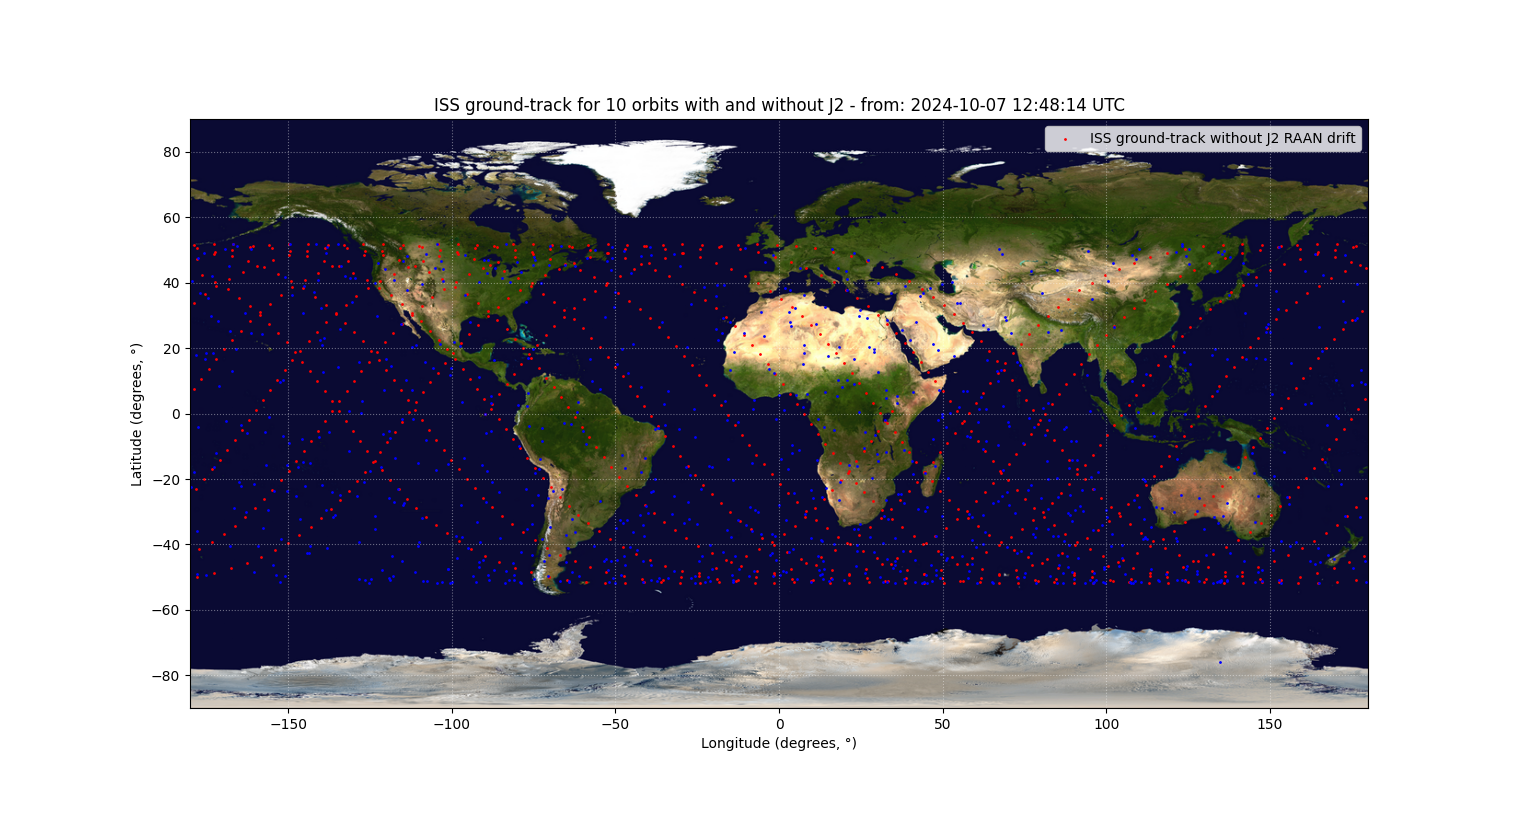
\includegraphics[width=1\linewidth]{Graphics/ISS_plot_J2.png}
    \caption{Plot of computed ISS orbit propagation ground track for 10 orbits without/with J2 using code from Appendix \ref{sec:Appendix_A}.}
    \label{fig:ISS_plot_J2}
\end{figure}